\documentclass[tikz,border=0cm]{standalone}

\usepackage[paperwidth=48in,paperheight=36in,margin=1in]{geometry}
\usetikzlibrary{calc}
\usetikzlibrary{decorations.pathmorphing,fit,arrows.meta,matrix}
\usepackage{qrcode}

% colors
\definecolor{ccmcyellow}{RGB}{254,196,54}
\definecolor{ccmcblue}{RGB}{8,65,96}
\definecolor{ccmcred}{rgb}{0.7,0.2,0.2}
\definecolor{icsyellow}{RGB}{254,223,101}

\definecolor{col1}{HTML}{fc9272}
\definecolor{col2}{HTML}{fee0d2}
\definecolor{col3}{HTML}{de2d26}
\definecolor{col4}{HTML}{4c72b0}
\definecolor{col5}{HTML}{dd8452}
\definecolor{col6}{HTML}{55a868}
\definecolor{col7}{HTML}{c44e52}

% fonts
%\usepackage{type1cm}
%\usepackage{cmbright}
\usepackage{fetamont}
\usepackage{fp}
\edef\myfontscale{1.4}
%% scalable vector fonts
\edef\fontSizeX{12}\edef\fontSizeY{14}
\FPupn{\resulttinyX}{myfontscale fontSizeX * 2 round}
\FPupn{\resulttinyY}{myfontscale fontSizeY * 2 round}
\renewcommand*{\tiny}{\fontsize{\resulttinyX}{\resulttinyY}\selectfont}

\edef\fontSizeX{14.4}\edef\fontSizeY{18}   
\FPupn{\resultscriptsizeX}{myfontscale fontSizeX * 2 round}
\FPupn{\resultscriptsizeY}{myfontscale fontSizeY * 2 round}
\renewcommand*{\scriptsize}{\fontsize{\resultscriptsizeX}{\resultscriptsizeY}\selectfont}

\edef\fontSizeX{17.28}\edef\fontSizeY{22}
\FPupn{\resultfootnotesizeX}{myfontscale fontSizeX * 2 round}
\FPupn{\resultfootnotesizeY}{myfontscale fontSizeY * 2 round}
\renewcommand*{\footnotesize}{\fontsize{\resultfootnotesizeX}{\resultfootnotesizeY}\selectfont}

\edef\fontSizeX{20.74}\edef\fontSizeY{25}
\FPupn{\resultsmallX}{myfontscale fontSizeX * 2 round}
\FPupn{\resultsmallY}{myfontscale fontSizeY * 2 round}
\renewcommand*{\small}{\fontsize{\resultsmallX}{\resultsmallY}\selectfont}

\edef\fontSizeX{24.88}\edef\fontSizeY{30}
\FPupn{\resultnormalsizeX}{myfontscale fontSizeX * 2 round}
\FPupn{\resultnormalsizeY}{myfontscale fontSizeY * 2 round}
\renewcommand*{\normalsize}{\fontsize{\resultnormalsizeX}{\resultnormalsizeY}\selectfont}

\edef\fontSizeX{29.86}\edef\fontSizeY{37}
\FPupn{\resultlargeX}{myfontscale fontSizeX * 2 round}
\FPupn{\resultlargeY}{myfontscale fontSizeY * 2 round}
\renewcommand*{\large}{\fontsize{\resultlargeX}{\resultlargeY}\selectfont}

\edef\fontSizeX{35.83}\edef\fontSizeY{45}
\FPupn{\resultLargeX}{myfontscale fontSizeX * 2 round}
\FPupn{\resultLargeY}{myfontscale fontSizeY * 2 round}
\renewcommand*{\Large}{\fontsize{\resultLargeX}{\resultLargeY}\selectfont}

\edef\fontSizeX{43}\edef\fontSizeY{54}
\FPupn{\resultLARGEX}{myfontscale fontSizeX * 2 round}
\FPupn{\resultLARGEY}{myfontscale fontSizeY * 2 round}
\renewcommand*{\LARGE}{\fontsize{\resultLARGEX}{\resultLARGEY}\selectfont}

\edef\fontSizeX{51.6}\edef\fontSizeY{64}
\FPupn{\resulthugeX}{myfontscale fontSizeX * 2 round}
\FPupn{\resulthugeY}{myfontscale fontSizeY * 2 round}
\renewcommand*{\huge}{\fontsize{\resulthugeX}{\resulthugeY}\selectfont}

\edef\fontSizeX{61.92}\edef\fontSizeY{77}
\FPupn{\resultHugeX}{myfontscale fontSizeX * 2 round}
\FPupn{\resultHugeY}{myfontscale fontSizeY * 2 round}
\renewcommand*{\Huge}{\fontsize{\resultHugeX}{\resultHugeY}\selectfont}

\edef\fontSizeX{74.3}\edef\fontSizeY{93}
\FPupn{\resultveryHugeX}{myfontscale fontSizeX * 2 round}
\FPupn{\resultveryHugeY}{myfontscale fontSizeY * 2 round}
\newcommand*{\veryHuge}{\fontsize{\resultveryHugeX}{\resultveryHugeY}\selectfont}

\edef\fontSizeX{89.16}\edef\fontSizeY{112}
\FPupn{\resultVeryHugeX}{myfontscale fontSizeX * 2 round}
\FPupn{\resultVeryHugeY}{myfontscale fontSizeY * 2 round}
\newcommand*{\VeryHuge}{\fontsize{\resultVeryHugeX}{\resultVeryHugeY}\selectfont}

\edef\fontSizeX{107}\edef\fontSizeY{134}
\FPupn{\resultVERYHugeX}{myfontscale fontSizeX * 2 round}
\FPupn{\resultVERYHugeY}{myfontscale fontSizeY * 2 round}
\newcommand*{\VERYHuge}{\fontsize{\resultVERYHugeX}{\resultVERYHugeY}\selectfont}

% set the normalfont (default)
\renewcommand*{\normalfont}{\normalsize}

\usepackage[none]{hyphenat}

\renewcommand*\familydefault{\sfdefault}
\usepackage[sfmath]{kpfonts}
\usepackage[T1]{fontenc}

\usepackage{amsmath,amssymb,bm}
\usepackage{wrapfig}
\usepackage{microtype}
\usepackage{booktabs}
\usepackage{siunitx}

\newcommand{\bs}[1]{\boldsymbol{#1}}
\newcommand{\ue}{u_\mathup{e}}
\newcommand{\Vm}{V_\mathup{m}}
\newcommand{\vV}{\mathbf{V}}
\newcommand{\vX}{\mathbf{X}}
\newcommand{\vZ}{\mathbf{Z}}
\newcommand{\vz}{\mathbf{z}}
\newcommand{\vx}{\mathbf{x}}
\newcommand{\vy}{\mathbf{y}}
\newcommand{\vw}{\boldsymbol{\xi}}
\newcommand{\vW}{\boldsymbol{\Xi}}
\newcommand{\vn}{\mathbf{n}}
\newcommand{\tA}{\mathbf{a}}
\newcommand{\tG}{\mathbf{G}}
\newcommand{\tI}{\mathbf{I}}
\newcommand{\tGi}{\tG_\mathup{i}}
\newcommand{\tGe}{\tG_\mathup{e}}
\newcommand{\tGb}{\tG_\mathup{b}}
\newcommand{\tGm}{\tG_\mathup{m}}
\newcommand{\Cm}{C_\mathup{m}}
\newcommand{\fion}{f_\mathup{ion}}
\newcommand{\R}{\mathbb{R}}
\newcommand{\dd}{\mathup{d}}
\newcommand{\EE}{\mathbb{E}}
\newcommand{\OmegaH}{\Omega_\mathup{H}}
\newcommand{\OmegaT}{\Omega_\mathu[{T}}
\newcommand{\Zlbar}{\bar Z_\ell}

\newcommand{\brho}{\bm{\rho}}

\newcommand{\sil}{\sigma_{\mathup{i},\mathup{l}}}
\newcommand{\sit}{\sigma_{\mathup{i},\mathup{t}}}
\newcommand{\sel}{\sigma_{\mathup{e},\mathup{l}}}
\newcommand{\set}{\sigma_{\mathup{e},\mathup{t}}}

\newcommand{\Vrest}{V_\mathup{rest}}
\newcommand{\Vthres}{V_\mathup{thr}}
\newcommand{\Vdepol}{V_\mathup{dep}}

\DeclareMathOperator{\Cov}{Cov}
\DeclareMathOperator{\Cor}{Cor}
\DeclareMathOperator{\Var}{Var}


\begin{document}

\begin{tikzpicture}[x=48in,y=36in]
\draw[blue!10!white,use as bounding box] (0,0) rectangle (1,1);


%%%% title %%%%
\begingroup
\pgfmathsetseed{3672}
\node[anchor=north west,fill=icsyellow,
text width=\paperwidth,inner sep=2cm,decorate,
decoration={random steps,segment length=1cm,amplitude=4mm},
draw=ccmcyellow,line width=2mm]
(title)
at ($(current bounding box.north west)+(-1cm,1cm)$)
{
{\ffmfamily\LARGE\bfseries
44: Fast and Accurate Uncertainty Quantification for the ECG With Random Electrodes Location}

\bigskip
{\bfseries
Michael Multerer, Pezzuto Simone
}

\raisebox{-2mm}{
\includegraphics[height=1em]{email}}
\texttt{michael.multerer@usi.ch}, \texttt{simone.pezzuto@usi.ch}

\bigskip
Center for Computational Medicine in Cardiology, Euler Institute,
Universit\`a della Svizzera italiana,\\
via la Santa 1, CH-6900 Lugano, Switzerland.
};
\endgroup

%%%%%%%%%%%%%%%%%%%%%%
%%%% introduction %%%%
%%%%%%%%%%%%%%%%%%%%%%

\tikzset{
  motif col/.style={inner sep=0.25in,text width=14.833in},
  motif title/.style={font=\bfseries\ffmfamily\Large},
}

\node[anchor=south west,motif title]
(motif title)  %at ($(title.south west)+(1.5cm,-3cm)$)
at ($(current bounding box.west |- title.south)+(0,-1.25in)$)
{Motivations};
\draw[line width=1mm] (motif title.south west) -- (motif title.south east);

\node[motif col,anchor=north west] (motif1) at
($(motif title.south west)+(1in,0)$)
{
The standard \textbf{surface ECG} is a valuable tool for assessing the
electric activity of the heart.  Routinely acquired and \textbf{non-invasive},
the ECG is also the perfect candidate for individualizing
\textbf{patient-specific models}.  As most clinical data, however,
the ECG is unavoidably subject to \textbf{uncertainty}.
};

\node[motif col,anchor=north west] (motif2) at (motif1.north east)
{
A simulated ECG is a point-wise evaluation of the potential on the chest.
Therefore, when the \textbf{location of the electrodes is not precise},
the signal is a random variable.  
Here we show how to \textbf{estimate the statistical moments} of
the ECG in a \textbf{very efficient} manner and suitable for model personalization.
};

\node[motif col,anchor=north west] (motif3) at (motif2.north east)
{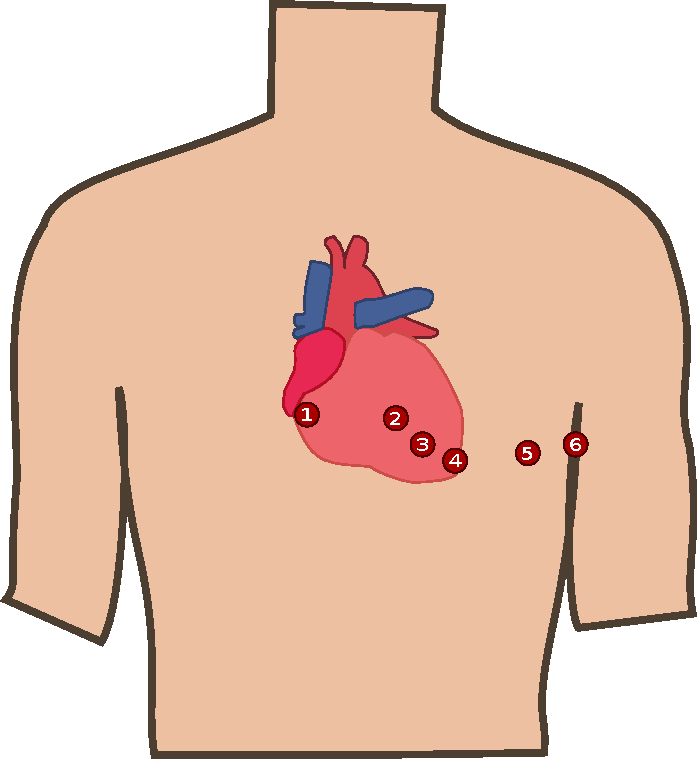
\includegraphics[width=3in]{img/torsoheart}\hfill
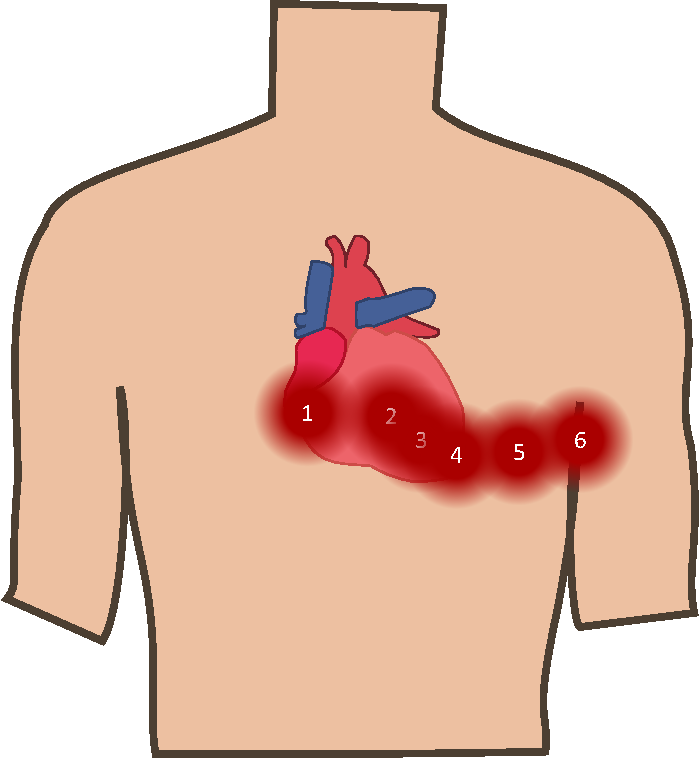
\includegraphics[width=3in]{img/torsoheart_rnd_crop}\hfill
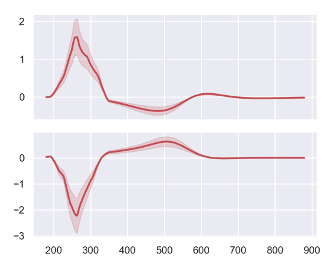
\includegraphics[width=7in,trim=0 0 0 60,clip]{img/ECG}
};

\node[fit={(motif1)(motif2)(motif3)},inner sep=0pt] (motif) {};

%%%%%%%%%%%%%%%%%
%%%% methods %%%%
%%%%%%%%%%%%%%%%%

\tikzset{
  hbox title/.style={draw=black,minimum width=15in,text=white,
                     fill=col4,rounded corners,font=\bfseries\ffmfamily},
  hbox main/.style={fill=col4!20!white,draw,rounded corners,fill opacity=0.9,
                    text opacity=1,,inner sep=0.25in,text width=14.5in,
                    text depth=11in,minimum height=11.5in},
  method title/.style={font=\bfseries\ffmfamily\Large},
}

\node[anchor=north west,method title] (methods title)
at ($(current bounding box.west |- motif.south)+(0,0.5in)$) {Methods};
\draw[line width=1mm] 
(methods title.south west) -- (methods title.south east);

%%% UQ PROBLEM %%%

\node[anchor=north west,hbox title]
(problem1 title) at ($(methods title.south west)+(1in,-0.5in)$)
{Problem statement};

\node[anchor=north west,hbox main]
(problem1) at ($(problem1 title.south west)+(0,-5mm)$)
{
\vspace{-5mm}\begin{itemize}
\renewcommand{\labelitemi}{$\blacktriangleright$}
\renewcommand{\itemsep}{1ex}

\item \textbf{Source of uncertainty}

The {\color{col3}\textbf{electrode locations}} on the chest.
Their position is a random vector
$\bs\Xi = \{ \bs\xi_1, \ldots, \bs\xi_L \}$ with
density $\rho(\vX)$.

\item \textbf{Quantity of interest}

The statistics of the ECG $V(t,\bs\Xi)$,
specifically the expectation $\EE[V](t)$ and
correlation $\Cor[V](t,s)$.

\item \textbf{Forward model}

Given the transmembrane potential $\Vm(\vx,t)$ on the heart $\OmegaH$,
we compute the ECG with the \textbf{\color{col3}forward bidomain model}
\[
- \operatorname{div}(\tG\nabla u) = \begin{cases}
\operatorname{div}(\tGi\nabla\Vm), & \mbox{on $\OmegaH$}, \\
0, & \mbox{otherwise}.
\end{cases}
\]

An ECG lead is a zero-sum linear combination of $u(\xi_\ell,t)$.

\item \textbf{Isn't it a simple integration problem?}

Yes, but a rather expensive one as the cost grows linearly with the
number of evaluations of the transmembrane potential $\Vm(\vx,t)$,
each requiring the solution of the elliptic PDE.

\end{itemize}
};

%%% LEAD FIELD FORMULATION %%%

\node[anchor=north west,hbox title,fill=col5]
(problem2 title) at ($(problem1 title.north east)+(0.5in,0)$)
{Lead field formulation and expectation};

\node[anchor=north west,hbox main,fill=col5!20!white]
(problem2) at ($(problem2 title.south west)+(0,-5mm)$)
{
\vspace{-5mm}%
%\begin{minipage}[t]{0.8\textwidth}
\begin{itemize}
\renewcommand{\labelitemi}{$\blacktriangleright$}
%\renewcommand{\itemsep}{1ex}

\item \textbf{Equivalent formulation}

The ECG is exactly represented by the formula
\begin{flalign*}
\quad& V(t,\bs\Xi) = \int_{\OmegaH} \tGi(\vx)\nabla\Vm(\vx,t) 
\cdot\nabla Z(\vx,\bs\Xi) \:\dd{\vx}, &&
\end{flalign*}
where $Z(\vx,\bs\Xi)$ is the \textbf{\color{col3}lead field}.

The formula is linear in $Z$, the only random \\
field. Hence, we focus on statistics of $Z$.

\item \textbf{Lead field problem}
\begin{flalign*}
\quad&\begin{cases}
- \operatorname{div}(\tG\nabla Z) = 0, & \mbox{in torso}, \\
- \tG\nabla Z\cdot\vn = \sum_i^L a_i \delta(\vx-\bs\xi_i), & \mbox{on chest}.
\end{cases} &&
\end{flalign*}

Note: the function $Z(\vx,\bs\Xi)$ is computed once!

\item \textbf{Expectation}

By linearity, we solve as above by replacing
\[
\begin{aligned}
V(\vx,\bs\Xi) &\quad\leadsto\quad \EE[V](t) \\
Z(\vx,\bs\Xi) &\quad\leadsto\quad \EE[Z](\vx) \\
\delta(\vx-\bs\xi_i) &\quad\leadsto\quad \rho_i(\vx)
\quad\mbox{(marginal distribution)}
\end{aligned}
\]

\end{itemize}

};
\node[anchor=north east] (lf) at ($(problem2.north east)+(-0.1in,-0.1in)$)
{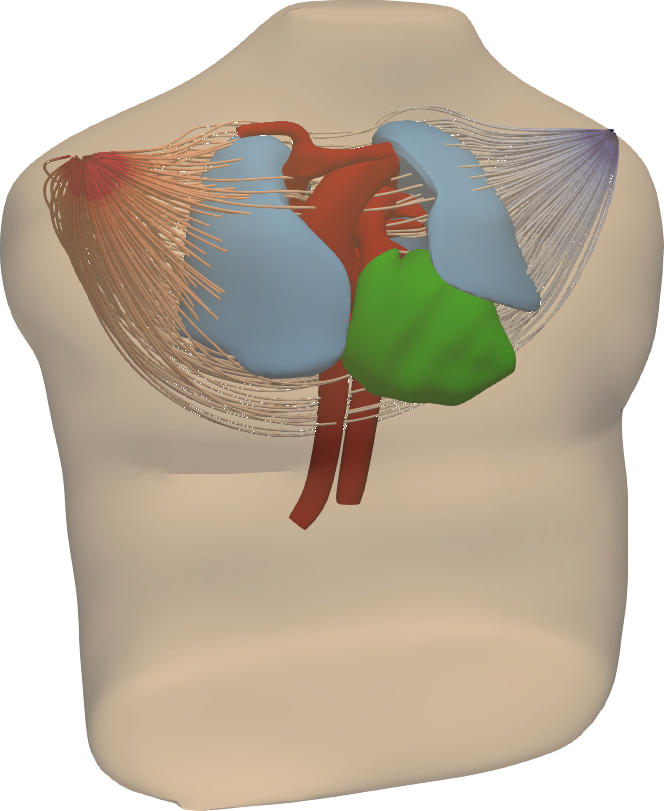
\includegraphics[width=3.5in]{img/CRT001_torsoLF_crop}}
node[anchor=north] at (lf.south) {\itshape Lead Field};


%%% COVARIANCE %%%

\node[anchor=north west,hbox title,fill=col6]
(problem3 title) at ($(problem2 title.north east)+(0.5in,0)$)
{Computation of ECG time correlation};

\node[anchor=north west,hbox main,fill=col6!20!white]
(problem3) at ($(problem3 title.south west)+(0,-5mm)$)
{
\vspace{-5mm}%
\begin{itemize}
\renewcommand{\labelitemi}{$\blacktriangleright$}
%\renewcommand{\itemsep}{1ex}

\item \textbf{Tensor product}

The correlation of the ECG is obtained by tensor product:
\[
\Cor[V](t,s) 
= \int_{\OmegaH^2} (\tGi\nabla\otimes\tGi\nabla) \Vm(\vx,t)\Vm(\vx',s)
: (\nabla\otimes\nabla) \Cor[Z]\: \dd\vx\dd\vx'.
\]

The correlation $\Cor[Z](\vx,\vx')$ of the lead field will
satisfy a problem obtained again from the tensor product 
of the lead field equation.  \textbf{\color{col3}The problem size is squared}.

\item \textbf{Low-rank approximation}

Since electrodes distribution is \textbf{\color{col3}highly localized},
we approximate the correlation with a low-rank tensor
\[
\Cor[Z](\vx,\vx') \approx \sum_{k=1}^K \zeta_k(\vx) \zeta_k(\vx'),
\qquad\mbox{$K$ small.}
\]

\item \textbf{Numerical solution}

In total, computing $\Cor[Z]$ amounts to the solution of $K$ elliptic
problems equivalent to the lead field problem (with different Neumann
data.)

\end{itemize}

};

\node[fit={(problem1 title)(problem1)
           (problem2 title)(problem2)
           (problem3 title)(problem3)},inner sep=0pt] (methods) {};

%%%%%%%%%%%%%%%
%%% results %%%
%%%%%%%%%%%%%%%

\node[anchor=north west,method title] (results title)
at ($(current bounding box.west |- methods.south)+(0,-0.5in)$)
{Numerical assessment};
\draw[line width=1mm] 
(results title.south west) -- (results title.south east);

\node[anchor=north west,inner sep=0.25in,text width=14.833in]
(res1 label) at ($(results title.south west)+(1in,-0.5in)$)
{\textbf{Problem setup:}
Idealized 2-D torso and an 2-lead ECG:
\[
\mbox{Lead II} = \mbox{VF} - \mbox{VL}, \qquad
\mbox{Lead V1} = \mbox{V1} - \tfrac{1}{3}\bigl(\mbox{VL} + \mbox{VR} + \mbox{VF}\bigr)
\]
};

\node[anchor=north west] (res1) at ($(res1 label.south west)$)
{\begin{tikzpicture}
    \def\myunit{6mm}
    \definecolor{colheart}{HTML}{fc9272}
    \definecolor{coltorso}{HTML}{fee0d2}
    \definecolor{colblood}{HTML}{de2d26}
    \definecolor{colVF}{HTML}{4c72b0}
    \definecolor{colVR}{HTML}{dd8452}
    \definecolor{colVL}{HTML}{55a868}
    \definecolor{colV1}{HTML}{c44e52}

    \definecolor{colgrid}{HTML}{f0f0f0}
    \tikzstyle{elec}=[circle,inner sep=10pt,draw=white,thin]
    \tikzstyle{heart}=[colheart,even odd rule,draw=black]
    \tikzstyle{torso}=[coltorso,draw=black,thick]
    \tikzstyle{tbox}=[rounded corners=1pt,fill=white,opacity=0.8,text opacity=1.0,
                      outer sep=2pt,font=\bfseries\sffamily\footnotesize]
    \tikzset{
    partial ellipse/.style args={#1:#2:#3}{
        insert path={+ (#1:#3) arc (#1:#2:#3)}
    }}
    % grid
    \fill[colgrid] (-11*\myunit,-16*\myunit) rectangle (11*\myunit,16*\myunit);
    \draw [step=5*\myunit,white,thick] (-11*\myunit,-16*\myunit) grid (11*\myunit,16*\myunit);
    % torso
    \fill[torso]  (0,0) ellipse [x radius = 10*\myunit, y radius = 15*\myunit];
    % heart
    \fill[colblood] (-4*\myunit,2*\myunit) circle[radius = 2*\myunit];
    \fill[heart] (-4*\myunit,2*\myunit) circle[radius = 3*\myunit] circle[radius = 2*\myunit];
    % electrodes
    \node[elec,fill=colVL] (VL) at ({10*\myunit*cos(deg(3*pi/4))},{15*\myunit*sin(deg(3*pi/4))}) {};
    \node[elec,fill=colVR] (VR) at ({10*\myunit*cos(deg(1*pi/4))},{15*\myunit*sin(deg(1*pi/4))}) {};
    \node[elec,fill=colVF] (VF) at ({10*\myunit*cos(deg(6*pi/4))},{15*\myunit*sin(deg(6*pi/4))}) {};
    \node[elec,fill=colV1] (V1) at ({10*\myunit*cos(deg(4*pi/4))},{15*\myunit*sin(deg(4*pi/4))}) {};
    % labels
    \node[tbox,right] at (VL.east) {VL};
    \node[tbox,right] at (VR.east) {VR};
    \node[tbox,above] at (VF.north) {VF};
    \node[tbox,below] at (V1.south) {V1};
    % arc-length
    \draw[thin] (9.8*\myunit,0) -- +(1.0*\myunit,0);
    \draw[thin,{Latex[length=3mm,width=5mm]}-] (0,0) [partial ellipse=-20:0:{10.4*\myunit} and {15.4*\myunit}];
    % legend
    \path (-10*\myunit,-18*\myunit) node[draw=black,fill=coltorso,label=right:{\footnotesize Torso}] (b1) {}
        +(7.5*\myunit,0) node[draw=black,fill=colheart,label=right:{\footnotesize Heart}] (b2) {}
       ++(15*\myunit,0) node[draw=black,fill=colblood,label=right:{\footnotesize Blood}] (b3) {};
\end{tikzpicture}};

\node[anchor=north west,inner sep=0pt,label=below:{\footnotesize $\blacktriangle$
Pdfs along curvilinear coordinate}]
(res2) at ($(res1.north east)+(1in,0)$)
{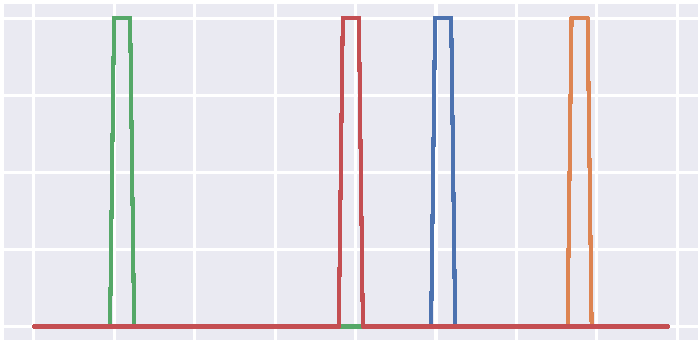
\includegraphics[scale=1.5]{img/rho_step_crop}};

\node[anchor=north,inner sep=0pt,label=below:{\footnotesize $\blacktriangle$
Activation map via eikonal}]
(res3) at ($(res2.south)+(0,-0.75in)$)
{
\includegraphics[scale=0.25]{img/activ}};

\node[anchor=north west,inner sep=0.25in,text width=14.833in]
(res4) at (res1 label.north east)
{\textbf{ECG results for all tests.}
In the plots, the dashed black curve
is the deterministic ECG, the solid blue curve is the average
ECG, and the shaded blue area corresponds to the \SI{95}{\percent} confidence
interval, that is $\EE[V](t) \pm  1.96\sqrt{\Var[V](t)}$.

\bigskip
\begin{center}
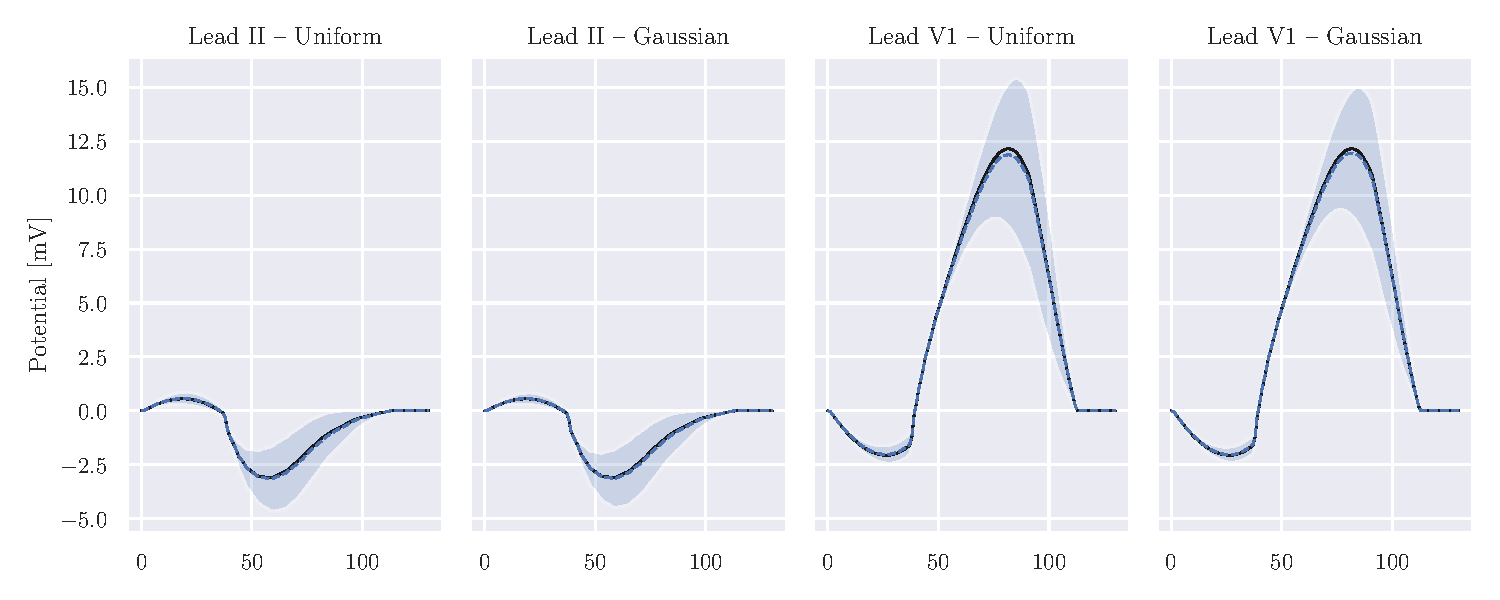
\includegraphics[width=0.9\textwidth,trim=10 10 10 10,clip]{img/ECGcomp.pdf}
\end{center}

\begin{itemize}
\renewcommand{\labelitemi}{$\blacktriangleright$}
%\renewcommand{\itemsep}{1ex}
\item \textbf{Low-rank modes} were 17 (lead II) and 33 (lead V1).

\item \textbf{Max std deviation} was 0.83\,mV (lead II) and 2.07\,mV (lead V1).

\item \textbf{High accuracy} to bidomain (error < 0.01\,mV).

\item \textbf{Computational cost} was 2- to 8-fold lower than bidomain.
\end{itemize}
};

\node[fit={(res1 label)(res2)(res3)(res4)},inner sep=0pt] (results) {};

%%%%%%%%%%%%%%%%%%%%
%%%% conclusion %%%%
%%%%%%%%%%%%%%%%%%%%

\node[anchor=north west,font=\bfseries\ffmfamily\Large]
(conclusions title) at ($(results title.north west -| results.east)+(0,-0.0in)$)
{Final remarks};
\draw[line width=1mm] 
(conclusions title.south west) -- (conclusions title.south east);

\node[anchor=north west,inner sep=0.25in,text width=13.833in]
(conclusions t1) at ($(conclusions title.south west)+(1in,-0.5in)$)
{
\vspace{-5mm}
\begin{itemize}
\renewcommand{\labelitemi}{$\blacktriangleright$}
%\renewcommand{\itemsep}{1ex}
\item We have solved the problem of quantifying the uncertainty
in the ECG when electrode positions is uncertain.

\item Our method recasts the
problem into a \textbf{fully deterministic setting} by using the
\textbf{lead field} theory and a \textbf{low-rank approximation} for the correlation.

\item \textbf{Computationally cheaper} than bidomain model,
cost independent of number of evaluations of $\Vm$.

\item Suitable to compute ECGs for \textbf{long simulations}, e.g., arrhythmic events,
and \textbf{inverse problems} involving the ECG.
\end{itemize}
};

%%% publist %%

\node[anchor=north west] (p1) at ($(conclusions t1.south west)+(1in,-0.5in)$)
{\qrcode[height=2in]{https://github.com/pezzus/fimh2021}}

node[anchor=west,text width=10in,draw] (p1 text) at (p1.east)
{
Try yourself on Jupyter!

\texttt{https://github.com/pezzus/fimh2021}.

(Full paper also available.)
};


%%%% logo %%%%
%\node[anchor=south west,inner sep=1cm]
%(logoICS) at (current bounding box.south west)
%{\includegraphics[height=5cm]{icslogo}};

\node[anchor=south east,inner sep=4mm]
(logoCCMC) at (current bounding box.south east)
{
\includegraphics[height=5cm]{ccmclogo}};

\node[anchor=north east]
(qrcode) at ($(current bounding box.north east)-(0.5in,0.5in)$)
{\qrcode[height=2in]{https://github.com/pezzus/fimh2021/blob/main/FIMH2021.pdf}};
\node[anchor=north east,text width=13cm,align=right]
(qrcode text) at (qrcode.south east)
{Download this poster! \\
(PDF format, $\sim$ 0.3\,MB)};

\end{tikzpicture}
\end{document}
